\section{Simulations}
\label{sec:sumulations}

\begin{figure*}[h]
\label{fig:regret_loss_scales}
\centering
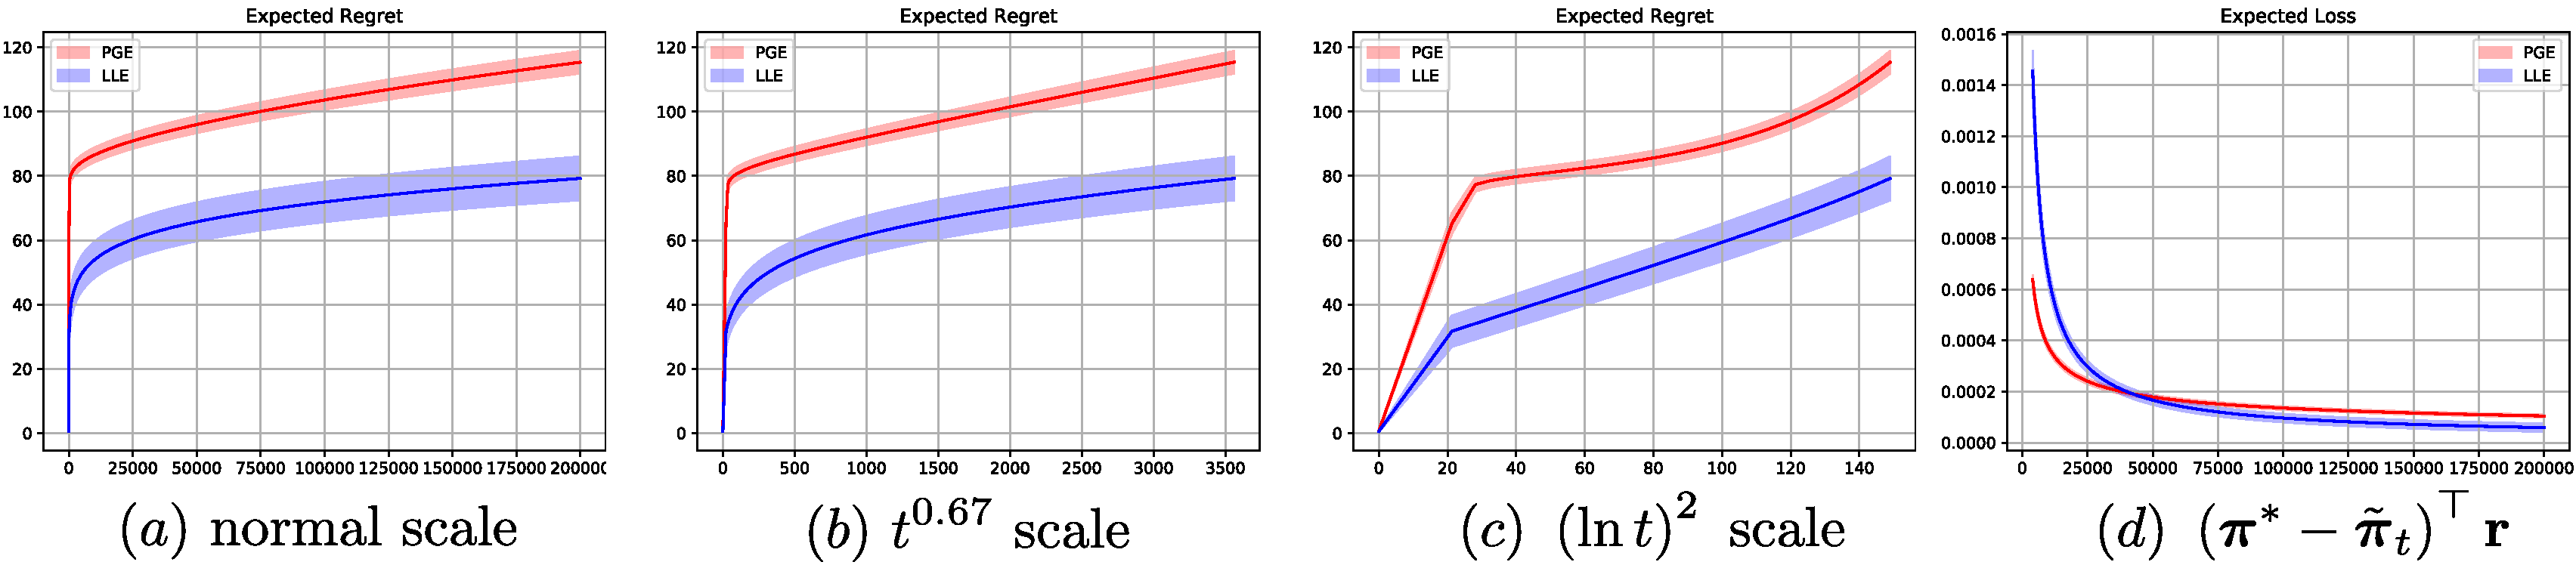
\includegraphics[width=1\linewidth]{comparison_PGE_LLE_regret_scales.pdf}
\caption{The regret of PGE and LLE in different scales, and the expected loss.}
\end{figure*}

We conducted experiments using the proposed PGE and LLE algorithms. The setting is $K = 50$, $m = 5000$, $d = 20$, and $T = 2 \times 10^5$. The true mean reward is uniformly generated $\rvr \in [0.0, 1.0]^K$, then the power $5$ is taken over $\rvr$. The standard deviation of each arm's reward is uniformly randomly generated in $[0.01, 0.05]$. The reward of each sampled action is then generated using a Gaussian distribution with the generated mean and standard deviation.

We repeatedly ran $10$ simulations. In each experiment, the true mean reward and variance are randomly generated. For PGE, $\frac{1}{3} - \beta$ is set to $0.33$, $\sigma = 0.0005$, and $\eta = 0.001$. For LLE, we use $\varepsilon_t = \frac{\ln{t}}{t}$, $\sigma = 0.002$, and $\eta = 0.0005$. At each step $t$, we calculate the expected regret $\sum\limits_{s = 0}^{t - 1}{ ( {\rvpi^*}  - \tilde{\rvpi}_s)^\top \rvr } $ and the latest expected loss $( {\rvpi^*}  - \tilde{\rvpi}_t)^\top \rvr$, where the expectation is taken over the mixed sampling policies in PGE/LLE.

As shown in \cref{fig:regret_loss_scales}, both PGE and LLE obtain expected regrets that are sub-linear in $T$. On the other hand, the expected regret of PGE decays much more slowly than that of LLE, since PGE has a large budget of $t^{\beta - \frac{1}{3}}$ for uniform exploration. We then scale the horizontal axis, to check whether the regret rates in theory are observable. In (b), in scale $t^{0.67}$, the regret of PGE scales almost linearly, indicating its expected regret is about $T^{\frac{2}{3}}$, which is consistent with \cref{thm:policy_gradient_main_result}. Similar results can also be observed for LLE and \cref{thm:logit_learning_main_result}, as shown in (c).
